\documentclass[10pt,twocolumn,a4paper]{article}

\usepackage{styles/usenix-style}
\usepackage{styles/ka-style}
\usepackage{xspace,ifthen,graphicx,listings}
\usepackage{styles/ka-style}

% \usepackage[utf8]{inputenc}
\usepackage[inline]{enumitem}
\usepackage{parskip} % disable indentation for new paragraphs, increased margin-bottom instead
\usepackage[english]{babel}
\usepackage{csquotes}
\usepackage[style=alphabetic]{biblatex}
\addbibresource{literature.bib}

\usepackage[binary-units=true]{siunitx}

\usepackage[
   pdfauthor={Christian Schwarz},
   pdftitle={Seminar Report - Light-Weight Contexts},
   pdfsubject={An OS Abstraction for Safety and Performance}, 
   pdfkeywords={}
]{hyperref}

\setlength{\marginparwidth}{2cm} % to make todonotes fit in twocolumn
\usepackage{todonotes}

\usepackage{blindtext}

\usepackage{listings}
\lstdefinestyle{lwcapi}{language=[ANSI]C,basicstyle=\ttfamily,basewidth=0.5em,fontadjust=true}
\lstset{style=lwcapi}

\lstdefinestyle{syscallinline}{float=h,aboveskip=-0.7em,belowskip=-0.7em}


\usepackage{diagbox}
\usepackage{multirow}

\usepackage{caption}
\usepackage{subcaption}

\usepackage{framed}

\usepackage{titlesec}
\titlespacing*{\section}{0pt}{1em}{0.25em}
\titlespacing*{\subsection}{0pt}{0.75em}{0.18em}
\titlespacing*{\subsubsection}{0pt}{0.5em}{0.12em}

\widowpenalty10000
\clubpenalty10000

\begin{document}

\title{%
  % document class article doesn't support subtitles, let's hack them
  {\normalfont \normalsize Seminar Report on}\\%
  Light-weight Contexts\\%
  {\normalfont \normalsize An OS Abstraction for Safety and Performance}\\%
  {\normalfont \small %
    James Litton\textsuperscript{1,2}
    Anjo Vahldiek-Oberwagner\textsuperscript{2}
    Eslam Elnikety\textsuperscript{2}
    Deepak Garg\textsuperscript{2}
    Bobby Bhattacharjee\textsuperscript{1}
    Peter Druschel\textsuperscript{2}
  }\\
  {\normalfont \small
    \textsuperscript{1}University of Maryland, College Park 
    \textsuperscript{2}Max Planck Institute for Software Systems
  }%
}
\author{%
Report by Christian Schwarz\\%
{\small Hot Topics in Modern Operating Systems}\\%
{\small ITEC, Karlsruhe Institute of Technology}\\%
{\small May -- August 2019}\\%
\vspace{1em}
}
\date{2019}

\maketitle

\begin{abstract}
Contemporary operating systems define processes as an execution environment for threads, consisting of a shared address space, file descriptor table, and system-level privilege.
The low overhead of threads compared to processes enables more efficient server applications, but prohibits meaningful memory isolation and privilege separation between potentially malicious requests.\\
Light-weight contexts (lwCs) provide an OS abstraction for privilege separation within a process by decoupling execution environment and logical control flow from processes and threads:
an lwC is comprised of an address space, file descriptor table and system credential, as well as one logical control flow per thread.
By allowing threads to rapidly switch between lwCs, pass arguments, and selectively share resources, compartmentalizing requests or code modules becomes possible.\\
In this report, we summarize the original lwC design and provide a brief analysis of its security model.
We proceed with a discussion of the authors' implementation and evaluation of lwCs on FreeBSD 11.0, pointing out substantial flaws and open questions with regards to real-world performance.
We conclude with a survey of related work in the field of application compartmentalization.
\end{abstract}

\section{Introduction}\label{intro}

% TODO NICE SUMMARY OF WHAT LWCs PROVIDE, CAN WE USE THIS ANYWHERE?
%Light-weight contexts can be used to create multiple protection domains within a single process,
%each with a private \textit{address space}, \textit{file descriptor table} and the system \textit{credential} and private per-thread logical control-flow %state (section~\ref{design:createdestroy}).
%Switching between the domains and single-value argument passing is controlled by the kernel (section~\ref{design:switching}).
%Dynamic sharing of resources between lwCs is also kernel-controlled using access capabilities (section~\ref{design:overlays}).
%Access to global namespaces \& system resources (IP sockets, file system, IPC) is limited by the lwC's \textit{credential} and can be further controlled %through syscall interposition (section~\ref{design:syscallinterpos}).
%
%Kernel-controlled switching between lwCs results in \textbf{well-defined entry points} under the assumption of an lwC created using \lstinline{COPY} resource %specifier\todo{this is quite coarse, AS and FDT sufficient?}:
%the first \lstinline{lwcSwitch} diverts physical control flow to the \lstinline{lwcCreate} call site in the new lwC, and all subsequent \lstinline{lwcSwitch}%es resume execution at an lwcSwitch all site.
%Under the assumption of no dynamic sharing, the address space of the target lwC is inaccessible to any caller.
%Thus, integrity and confidentiality guarantees for code and data within an lwC are those of the application code creating the lwC and those of the code %executing in the target lwC after \lstinline{lwcSwitch}.
%The result is a narrow, auditable interface.
%

Modern application architecture emphasizes modularization and information hiding to achieve testability, maintainability, exchangability, and reusability.
Type systems, packaging hierarchies, and visibility features in many programming languages can help to enforce said principles in large applications.

However, there is a chasm between the way we architect software and the way it is executed it at runtime:
whereas the programming language enforces strict separation between modules at compile time,
the program binary or interpreted script executes in a single protection domain --- the process ---
with shared address space, file descriptor table and system-level privilege for all modules.
Consequently, an exploitable vulnerability in a single logical module can be used to compromise the entire application, extract user data from application memory or serve as a basis for further privilege escalation.

Language technology provides holistic solutions to this problem, but performance concerns, lack of interoperability between different source languages, and legacy code bases shift the search for better runtime safety guarantees toward the next lower layer of the software stack:
can the operating system provide an efficient abstraction to maintain some of the aforementioned compile-time isolation at runtime?

Light-weight contexts (lwCs) are such an OS-based solution that allows for multiple protection domains (\textit{contexts}) within the same process:
An lwC is comprised of an address space, file descriptor table and system credential (privilege level).
In contrast to the implicit execution environment provided by a process, lwCs are a first-class OS abstraction and explicitly tangible from user space as file descriptors.
\cite{lwcpaper}

In the proposed design, threads no longer execute a single logical control flow, but have one \textit{per lwC}.
A new system call allows for rapid voluntary switching to a different lwC: apart from resuming the thread's logical control flow, the system call also installs the target lwC's address space, file descriptor table and system credential for the current thread.
Argument passing functionality on switch then enables the decomposition of an application's functionality into multiple lwCs that can provide independent security guarantees.
\cite{lwcpaper}

LwCs are created as snapshots of the current lwC's address space, file descriptors and privilege level.
Dynamic sharing of these resources is also supported through a capability system built on top of lwC file descriptors.
Privilege escalation through out-of-process channels can be prevented using syscall interposition.
\cite{lwcpaper}

The authors provide an evaluation of their implementation in FreeBSD 11.0, focusing on the enhancement of inter-request isolation and TLS private key protection in web servers.
Whereas the presented results are impressive at first glance, we find that the evaluation lacks key metrics for the presented use cases and does not sufficiently investigate obvious performance constraints of the design.

% Generic questions / problems / tradeoffs:
% \begin{itemize}
  % \item threat model
  % \item definition of what makes a protection domain
  % \item how to integrate the decomposition into different protection domains into the PL / runtime?
  % \item applicability to existing PLs \& code bases
  % \item how to maintain application performance
% \end{itemize}

\subsection{Structure of this Report}
This report provides a summary of the original light-weight context paper enriched with several insights drawn from the authors' open source implementation.
Section~\ref{design} provides an overview of the design and system API exposed by lwCs,
followed by a brief security analysis in Section~\ref{security}.
We give an overview of the changes made to FreeBSD 11.0 in order to support lwCs in Section~\ref{impl} and proceed with a discussion of the evaluation results of the original paper (Section~\ref{eval}).
Subsequently, we provide an elaborate critique of the design \& evaluation in Section~\ref{eval:crit}.
Finally, we survey other approaches to application compartmentalization in Section~\ref{rel}.

\begin{figure*}[t]
  \centering
  % \hfill
  \subcaptionbox{
      \textbf{Canonical model}\hspace{1em}
      The process impicitly defines the execution environment for threads.
      Threads are scheduling entities that represent a single control flow bound to the process-defined environment.
    \label{design:fig:canonicalprocthreads}
  }
  [0.4\linewidth]
  {
    % \centering
    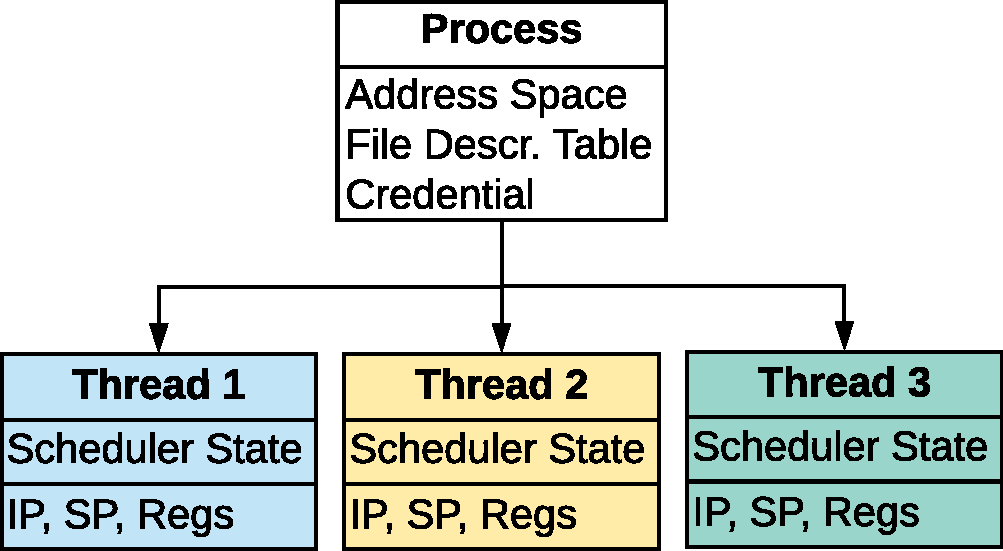
\includegraphics[width=\linewidth]{fig/canonical-proc-thread-relationship}
  }
  \hspace{1cm}
  \subcaptionbox
  {
      \textbf{lwCs}\hspace{1em}
      Processes act as containers for threads and lwCs.
      Threads are still scheduling entities, but have one logical control flow \textit{per lwC}.
      The lwC defines the execution environment for each thread and its logical control flow within the lwC.
    \label{design:fig:lwcprocthreadrelationship}
  }
  [0.4\linewidth]
  {
    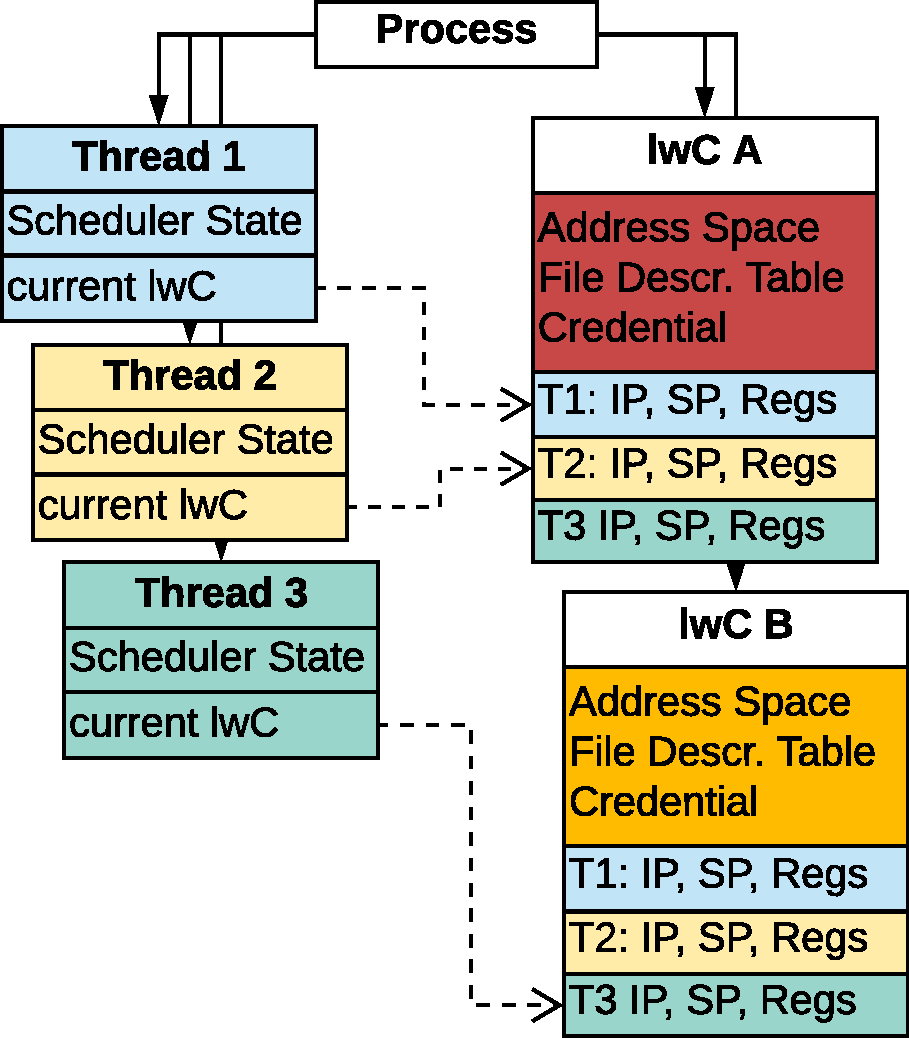
\includegraphics[height=6cm]{fig/lwc-proc-thread-relationship}
  }
  \caption{Canonical processes and threads vs. the lwC design.}
\end{figure*}


\section{Design}\label{design}


We find it most helpful to develop the general idea of light-weight contexts by starting from the canonical abstraction of processes \& threads, as visualized in Figure~\ref{design:fig:canonicalprocthreads}:
Conventionally, processes define an execution environment which is shared by one or more threads.
The execution environment consists of an address space, a file descriptor table and a representation of the process's system-wide privileges (\textit{credential}).
Threads have two roles within a process:
\textbf{first}, they represent \textbf{single units of logical control flow} within the process-defined environment.
Control flow has associated state, e.g., instruction pointer, stack pointer, general purpose register contents, FPU state, etc.
That state resides in a CPU's registers while the thread is executing, or in the thread control block (TCB) when off CPU.
The \textbf{second} role of a thread is that of a \textbf{scheduling entity}:
The scheduler time-multiplexes threads onto CPU cores and implements the concept of blocking and waiting between threads.
The scheduler state required for this task is stored in the TCB.

The authors introduce lwCs as a new OS abstraction and restructure the roles of canonical processes and threads, as visualized in Figure~\ref{design:fig:lwcprocthreadrelationship}:
\begin{itemize}
\item An lwC represents a single protection domain (address space, file descriptor table and system-wide privilege) and all logical control flows within that protection domain.
\item Threads always execute within one lwC at any given time and always execute the same logical control flow while within that lwC.
\item Multiple threads can execute simultaneously within an lwCs, sharing a protection domain but executing different logical flows.
\item lwCs are represented as file descriptors, and thus explicitly tangible from user space.
\item Threads can switch protection domains and logical control flow by switching between lwCs.
\end{itemize}
\cite{lwcpaper,lwckernelrepo}

In the following subsections, we provide an outline of the system API for managing and using lwCs in an application.

\subsection{lwC Switching}\label{design:switching}
We start our survey of the lwC API surface with the most central functionality: switching between lwCs.
We accept the existence of multiple lwCs for now and come back to lwC creation in the next subsection.

Threads can switch between lwCs by invoking the \lstinline{lwcSwitch} system call:

\begin{lstlisting}[style=syscallinline]
  caller, carg := lwcSwitch(target, arg) 
\end{lstlisting}

The first argument \lstinline{target} specifies the file descriptor of the lwC into which the calling thread wants to switch.
When invoking the system call, the kernel
\begin{enumerate}[nosep,label=(\alph*)]
\item saves the current control flow state into the current thread's lwC,
\item atomically switches to the new protection domain by installing the target lwC address space, file descriptor table and credential for the current thread,
\item and restores the control flow state saved for the current in thread in the target lwC.
\end{enumerate}
\cite{lwckernelrepo,lwcpaper}
% Pseudo code for this procedure is provided in Figure~\ref{design:fig:switchpseudocode}.

% \begin{figure}[b] % TODO drop this
%   \begin{lstlisting}[basicstyle=\footnotesize\ttfamily,mathescape,frame=single,linewidth=0.9\linewidth,belowskip=0pt,aboveskip=0pt,xleftmargin=0.05\linewidth]
%     syscall
%     SP, IP, $\dots$ $\rightarrow$ curLWC->tcb[tid]
%     curThd->vmspace = targetLWC->vmspace
%     curThd->fdt = targetLWC->fdt
%     curThd->cred = targetLWC->cred
%     curLWC = targetLWC
%     SP, IP, $\dots$ $\leftarrow$ targetLWC->tcb[tid]
%     (arg kept in register)
%     sysret  
%   \end{lstlisting}
%   \caption{Pseudo code for lwcSwitch.}
%   \label{design:fig:switchpseudocode}
% \end{figure}

It is crucial to understand that \textbf{execution after a switch always resumes at an lwC call site}, except for the very first switch into a newly created lwC (see next section).
This behavior is analogous to a voluntary context switch, e.g., with \lstinline{pthread_yield}.
However, in contrast to the canonical model of processes and threads, \textbf{\lstinline{lwcSwitch} does not switch to another scheduling entity}:
from the scheduler's perspective, it is still the same scheduling entity that is executing on the CPU.
Regular context saving and restoration after interrupts, exceptions or when a thread blocks, is left unchanged.
Only the memory location for off-cpu control flow state changes from the thread's control block to the thread's slot in the current lwC.
\cite{lwckernelrepo}

The second argument to \lstinline{lwcSwitch} is the opaque value \lstinline{arg} which is passed through to the code that starts executing in the target lwC after the switch.
The C bindings make that value available in the first return value \lstinline{carg}.
The second return value \lstinline{caller} is the file descriptor of the lwC from where the switch was initiated.
\cite{lwcpaper}

In summary, \lstinline{lwcSwitch} combines three tasks in one operation: kernel-moderated control flow switching, protection domain switching, and argument passing.
This combination enables the construction of lwCs that fulfill a server-like role within an application, providing independent security guarantees:
an lwC can implement high-assurance functionality in a private address space and enforce specific entry-points (\lstinline{lwcSwitch} call sites) where argument validation can be performed.

\subsection{lwC Creation \& Destruction}\label{design:createdestroy}
A process in an lwC system starts with a single thread that executes within a root lwC created by the OS.
This design enables backwards binary-compatibility with the exception that the root lwC file descriptor is a well-known number analogous to those for stdio.
\cite{lwcpaper}

New lwCs can be created from any thread with the \lstinline{lwcCreate} system call shown in Figure~\ref{design:fig:lwcCreate}.
By default, a new lwC is a snapshot of the calling thread's current lwC, as depicted in Figure~\ref{design:fig:lwccreationsequencediagram}:
The kernel first creates copies of the resources \textit{address space}, \textit{file descriptor table} and \textit{credential} and stores them in the new lwC.
It then temporarily preempts all threads that execute in the current lwC and stores their control flow state in the new lwC.
Finally, the file descriptor referring to the new lwC is returned to user space in the return value \lstinline{new}.
\cite{lwcpaper}

\begin{figure}
  \centering
  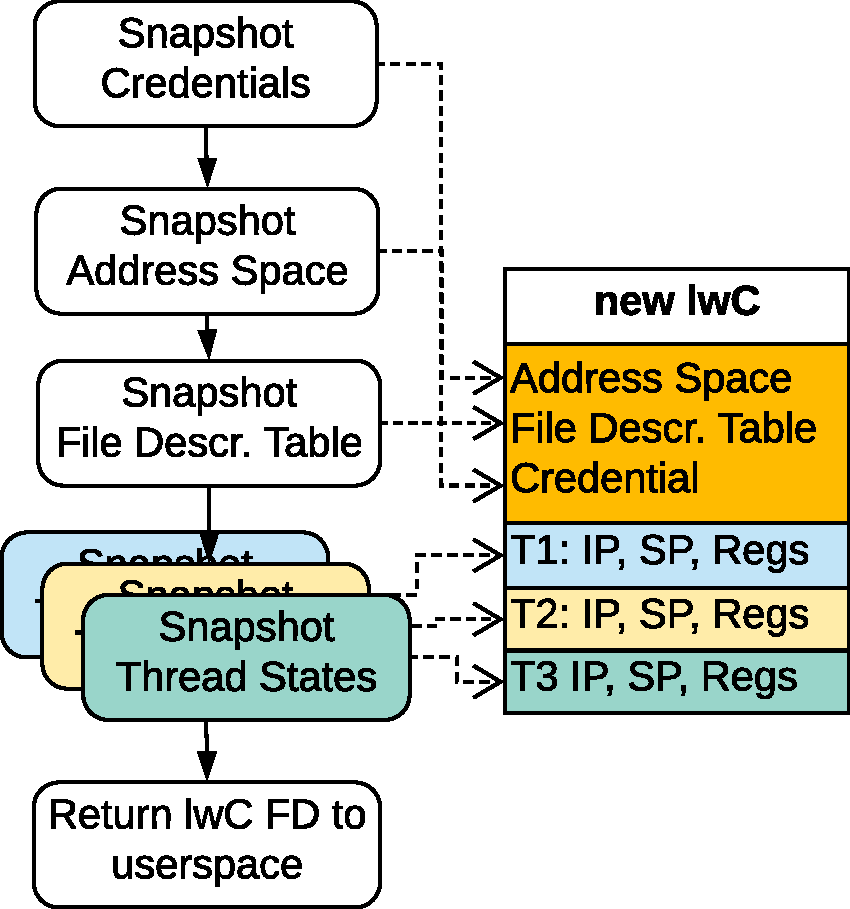
\includegraphics[height=6cm]{fig/lwc-creation-sequence-diagram}
  \caption{
    Steps involved in lwC creation.
    By default, a new lwC is a copy (snapshot) of the current lwC's resources.
    All threads that exist at the time of lwC creation can enter the new lwC.
  }
\label{design:fig:lwccreationsequencediagram}
\end{figure}

Although this procedure resemmbles the \lstinline{fork} system call, it is crucial to understand that no new process or scheduling entity is created.
\lstinline{lwcCreate} merely snapshots the current protection domain and provides a handle for existing threads to resume execution at that snapshot through \lstinline{lwcSwitch}.

Still, one problem of forking translates to lwC creation:
what happens on the first switch into a newly created lwC?
After all, the first \lstinline{lwcSwitch} already expects the target logical control flow to be at an \lstinline{lwcSwitch} call site.
We distinguish between the creating thread and other threads in the process:
the creating thread returns \enquote{a second time} from that syscall and populates \lstinline{lwcCreate}'s \lstinline{caller} and \lstinline{carg} return values with those of \lstinline{lwcSwitch}.
The additional return value \lstinline{new} contains the lwC descriptor of the creator lwC.
The behavior in the creating thread is thus well-defined.
The second case covers other threads, which could be at random points in their logical control flow when being snapshotted.
Switching to such threads generally results in undefined behavior and must be prevented by developers using barrier-synchronization.~\cite{lwcpaper}
However, it is unclear to us how the \lstinline{caller} and \lstinline{carg} return values are accessible to non-creator threads without inline-assembly or language support.

Note that a new lwC only stores control flow states for the threads that existed at the time of its creation:
threads created after the lwC cannot switch into the lwC.

\vspace{1.5em}
\begin{figure}[h]
  \centering
  \begin{framed}
\begin{lstlisting}[mathescape,aboveskip=0pt]
  new, caller, carg := lwcCreate(rspecs)
\end{lstlisting}
\begin{tabular}{|r||c|c|c|}
  \hline
                &   new        & caller       & carg \\
  \hline\hline
  creator       & new lwC fd   & $\bot$      & $\bot$\\
  \hline
  new lwC       &    creator lwC fd   & \multicolumn{2}{c|}{like lwcSwitch}\\
  \hline
\end{tabular}
\end{framed}
\caption{
  \texttt{lwcCreate} return values are different in creator and new lwC to ensure well-defined behavior when the creator switches to the new lwC for the first time.
  \label{design:fig:lwcCreate}
}
\end{figure}


\subsubsection{lwC Resource Specifiers}\label{design:rspecs}
The previous section presented the default behavior of \lstinline{lwcCreate} for an empty \lstinline{rspecs} argument.
By default, a new lwC is a snapshot copy of the current lwC's resources \textit{address space}, \textit{file descriptor table} and \textit{credential}.
However, it can also be desirable to share memory areas with the new lwC for bulk data tranfer, or to unmap memory from the new lwC to keep data secret.

\textit{Resource specifiers} provide fine-grained control of the resource sharing on \lstinline{lwcCreate}:
callers can specify per resource-kind whether the resource shall be \textit{copied to}, \textit{unmapped from} or \textit{shared} with the new lwC.
Address space and file descriptor sharing can be be specified on a per-page or per-descriptor basis.
Figure~\ref{design:fig:rspectable} summarizes the different combinations of resources and sharing behavior.
\cite{lwcpaper}

\begin{figure*}[h]
\begin{lstlisting}[xleftmargin=0.4\linewidth]
rspecs := [{Resource , [Start, End), How}]
\end{lstlisting}
\centering
\begin{tabular}{|r||c|c|c|}
  \hline
  \diagbox[width=5em]{How}{What}    &     Address Space         &         File Descriptor Table         &           Credential           \\
  \hline\hline
  COPY                              &   copy on write sharing           &      \texttt{dup} open FDs once    &  copy credential kobject  \\
  \hline              
  UNMAP                             &   do not map              &       do not \texttt{dup} FDs         &    $\bot$       \\
  \hline              
  SHARE                             &   shared memory            &   share kobject   &             share kobject   \\
  \hline
\end{tabular}
\caption{
  Resource specifiers change the default snapshot semantics of \texttt{lwcCreate}:
  each resource can be copied, shared or unmapped from the new lwC.
  Address space and file descriptor sharing can be configured per page or per descriptor.
  \textit{COPY} sharing is roughly equivalent to what happens on \texttt{fork}, \textit{SHARE} to what happens on thread creation.
  }
\label{design:fig:rspectable}
\end{figure*}

\subsection{Dynamic Resource Sharing}\label{design:overlays}
Apart from sharing resources at lwC creation time, it is also possible to dynamically copy or share memory and file descriptors between lwCs using the the \lstinline{lwcOverlay(src, rspecs)} system call.
The \lstinline{src} argument is the lwC descriptor of the lwC from which the subset of resources specified in \lstinline{rspecs} should be mapped (\textit{overlaid}) into the current lwC.
%The target address, or file descriptor number, respectively, is guaranteed to be the same as in \lstinline{src}.
To unmap an existing overlay, \lstinline{src} must be set to the current lwC and \lstinline{rspecs} must be filled with \lstinline{UNMAP} resource specifiers. 
%Overlays do not support stacking: after unmapping an overlay that overlaid an existing memory mapping, that original memory mapping is not automatically remapped.  %vmspace_lwc_merge
System credential overlays enable temporary privilege escalation to the credential of the \lstinline{src} lwC.
\cite{lwcpaper}

Overlays are subject to a \textbf{access capability system}:
the lwC descriptor kernel representation (\lstinline{struct filedescent}) carries an rspec-like mask that represents permitted overlays.
\lstinline{lwcOverlay} checks that the requested overlay \lstinline{rspec} is a subset of the permitted-overlay mask.
The \lstinline{lwcRestrict(target, rspecs)} system call allows reduction (but not addition) of overlay permissions:
given an lwC descriptor \lstinline{target}, \lstinline{lwcRestrict} removes the \lstinline{rspecs} from the mask, prohibiting future overlays through \lstinline{target}.
The capability system is bootstrapped by equipping the \lstinline{new} descriptor returned to the caller of \lstinline{lwcCreate} with a universal access capability to the child lwC.
The creator can also allow overlays of its resources by the child by setting a flag %\lstinline{LWC_MAY_ACCESS}
in the \lstinline{lwcCreate} \lstinline{rspecs} argument. 
\cite{lwckernelrepo,lwcpaper}

\subsection{Syscall Interposition}\label{design:syscallinterpos}
% kernel: lwctrapto in sys/kern/subr_syscall.c basically just calls lwcswitch 
It can be desirable to limit the system calls an lwC may perform, e.g., to limit file system access to a subdirectory, prohibit network communication, or avoid privilege escalation through other system calls.  
The lwC design builds onto existing syscall filtering and mechanisms, e.g. Capsicum capability mode on FreeBSD or seccomp on Linux:
when an lwC is created with the \lstinline{LWC_TRAP_SYSCALL} flag, system calls made by the new lwC or any of its children that would normally trap due to the syscall filtering mechanism are redirected to the creator as an \lstinline{lwcSwitch}.
The \lstinline{caller} return value of \lstinline{lwcSwitch} is set to the trapping lwC and \lstinline{cargs} contains the syscall arguments for inspection by the trap-handling lwC.
\cite{lwcpaper}

The trap-handling lwC can use the \lstinline{lwcSyscall} syscall execute a system call \textbf{in the context of the trapping lwC}:
the \lstinline{mask} argument allows the trap-handling lwC to choose per resource type whether its own resource mapping or that of the trapping lwC should be used while the syscall is executed.
It is further possible to make \lstinline{lwcSyscall} return to the trapping lwC on completion of the syscall.
Both options are optimizations that avoid temporary overlays and additional context switches.
\cite{lwcpaper,lwckernelrepo}

\begin{lstlisting}[style=syscallinline]
  lwcSyscall(trappingLwc, mask,
             syscall, syscall-args)
\end{lstlisting}

\subsection{Signal Delivery}
UNIX signal delivery with lwCs faces similar design questions as signal delivery in multi-threaded applications: To which lwCs should a given signal be delivered?
The authors' solution is classification of signals as either \textit{attributable} or \textit{non-attributable}:
attributable signals such as for segmentation faults are always delivered to the thread in the lwC that caused the signal to occur.
Non-attributable signals are delivered to \textit{all} lwCs created with a corresponding flag.
If a thread executes in a different lwC, signal delivery is deferred until that thread switches to the signalled lwC.
\cite{lwcpaper}
%We assume that above delivery model requires separate signal masks per lwC and thread.

\subsection{Forking \& Exit}
A forked process inherits the parent's lwCs.
However, only the forking thread exists in the child process, presumably due to POSIX compliance\cite{forkmultithread}. %read do_fork, which calls copy_snaps
Shared memory established through \lstinline{lwcCreate}, \lstinline{lwcOverlay}, or \lstinline{mmap(..., MAP_SHARED)} stays shared across forks.
The authors do not specify the behavior for file descriptor tables and credential; we assume unmodified fork semantics per lwC.
\cite{lwcpaper}

The exit system call terminates the entire process, regardless of the lwC in which it was called.
Syscall interposition can be used to avoid this specific problem, but process-wide denial of service from within a compromised lwC cannot be fully avoided, which we will discuss in the next section.
\cite{lwcpaper}


\section{Security Analysis}\label{security}

In this section, we define a threat model for lwCs and assess how the design meets the canonical information security properties of \textit{confidentiality}, \textit{integrity} and \textit{availability}~\cite{ciagoals}.

\textbf{Threat Model}\hspace{1em}
The run-time trusted computing base of a process that uses light-weight contexts is the
hardware,
firmware,
monolithic OS kernel,
any user space processes able to influence the execution of the lwC-process,
and any user space code that runs before \lstinline{main} starts executing.
Once \lstinline{main} starts executing, we assume an attacker who is able to hijack control flow and execute arbitrary code in user-mode in the currently established execution context, i.e., the current lwC.
Specifically, an attacker may access any mapped memory through unprivileged instructions and invoke any system call, including lwC management calls, and attempt privilege escalation directly or indirectly by invoking said system calls.
\cite{lwcpaper}

\textbf{Resource Mappings}\hspace{1em}
The kernel implementation of \texttt{lwcSwitch} must guarantee that all kernel subsystems as well as the memory management unit (MMU) will always perform their respective access permission checks against the resource mappings of the lwC that was last switched to, i.e., the current thread's current lwC.
Under that assumption, the lwC security guarantees rely solely on the soundness of the rules by which resource mappings can be manipulated from user space through \lstinline{lwcCreate}, \lstinline{lwcRestrict} and \lstinline{lwcOverlay}.
With regards to static resource sharing, the rules are sound if access to a parent lwCs or its data can only be reduced along an lwC creation chain.
For dynamic resource sharing, the semantics defining soundness depend on the use case and thus cannot be given or proven generally.
Neither the original paper's authors nor us provide a proof of soundness of the resource mapping manipulation.

The \lstinline{lwcSyscall} API must be considered separately:
its \lstinline{mask} argument allows the trap-handling lwC to specify a \textit{combination} of resource mappings of the trapping and trap-handling lwC for the duration of the syscall.
This differs from \lstinline{lwcSwitch}, which only allows switching \textit{all three resource mappings} atomically before executing code in the context of the target lwC.
It is the application developer's responsibility to ensure that the resource combination is compatible with the semantics behind the syscall's permission checks when using this mechanism.


\textbf{Achieving Protection Goals}\hspace{1em}
Applications must create lwCs with correct resource mappings and access capabilities in order to achieve their desired protection goals.
For example, full confidentiality and integrity of a region of memory in the root lwC can be achieved by asserting that all child lwCs are created with a resource specifier that marks that respective memory region as \lstinline{UNMAP}ped.
\enquote{Loop holes} such as attaching a debugger to the parent lwC from the child lwC must also be addressed, e.g., through system call interposition or by dropping privileges in the child lwC.

We believe that unintended is a highly-probable risky programming error due to the default copy-on-write sharing on lwC creation.
Unintended access right propagation or information flow through overlays at runtime might be even more difficult to spot in code reviews or audits.
Therefore, the authors recommend to use overlays \enquote{carefully} \cite{lwcpaper}.

Availability cannot be guaranteed by lwCs:
an attacker in control of an lwC can invoke the \lstinline{exit} system call to terminate the process unless syscall interposition is used to prevent that syscall.
Also, an attacker may modify the code in a compromised lwC to trap all threads that switch to it.
The authors dismiss both problems by describing denial-of-service (DoS) within a process as \enquote{self-defeating}.
\cite{lwcpaper}
We remark that the original paper does not address per-lwC resource usage (limits), which could serve as another DoS vector. 



% \subsection{Example Use Case: Application Compartmentalization}\label{design:usage} % TODO drop

% Application developers can leverage lwCs to achieve application protection goals.
% We restrict ourselves to an example use case for lwCs of a fictional application called \newcommand\appname{\textit{cnvrt}\xspace} \appname.
% We are going to use lwCs for \textit{compartmentalization} to increase confidentiality of user data and the server's TLS private key. 
% \appname is a network service which
% \begin{enumerate}[nosep]
%   \item starts a TLS server which accepts connections from arbitrary clients on the Internet,
%   \item reads a JPEG images over established connection,
%   \item uses an image processing library to convert the image into the client-requested output format and
%   \item sends a response with the converted image back to the client.
% \end{enumerate}

% We consider an attacker who exploits a vulnerability in the image processing library's image codec parser to achieve remote code execution:
% in an uncompartmentalized design, a successful attacker can read the entire process's memory to extract the private key of the TLS key pair or access other users' images from other requests.
% Both \textit{private key confidentiality} as well as \textit{client session isolation} are compromised.

% In contrast, an lwC-enabled design loads the TLS private key into the root lwC and waits for connections.
% For each new connection, it creates a worker lwC with private copy of the root lwC's address space and file descriptor table and switches into it.
% After performing the TLS hand-shake, it erases the private key from the worker address space and, only then, starts executing the riskier image processing code.
% A successful attacker has no longer access to the private key and is limited to the socket representing their own connection, as well as their own request data.
% A visualization of the compartmentalized design is given in Figure~\ref{design:usage:apparchpost}.

% \begin{figure}
%   \centering
%   \missingfigure[figheight=5cm]{Visualize \appname control flow, similar to the one in the seminar presentation bonus slides.}
%   \caption{
%     The compartmentalized \appname application uses a separate lwC for the initial TLS handshake to protect the private key and per-request lwCs to isolate concurrent requests from each other.
%     \label{design:usage:apparchpost}
%   }
% \end{figure}

% Note that we have constructed a simplified example where requests can be handled in full isolation.
% In practice, some sharing will be required, e.g., for global statistics, a database connection pool, logging services, etc.
% In an lwC-compartmentalized design, these components would execute in separate lwCs and be made accessible to the worker lwCs via shared memory, \lstinline{lwcSwitch}, \lstinline{lwcOverlay} or traditional IPC mechanisms.

% Note further that we have not discussed the concurrency model of \appname:
% both threaded and event-driven models are possible, as will be explained briefly in Section~\ref{eval:web}.


\section{Implementation}\label{impl}

The authors implement lwCs in the FreeBSD 11.0 operating system and make the source code publicly available.~\cite{lwckernelrepo,lwclibsrepo} % see literature.bib for git diff
The major changes to the kernel consist of:
\begin{itemize}[nosep]
  \item An implementation of lwC management syscall handlers and resource specifier logic.\\
  +2388 lines in \texttt{sys/sys/kern\_snap.c}
  \item Support for resource specifiers and overlays in the file descriptor management and memory management subsystem.\\
  +251 lines in \texttt{sys/kern/kern\_descrip.c}\\
  +693 lines in \texttt{sys/vm/vm\_map.c}\\
  +178 lines in \texttt{sys/amd64/amd64/pmap.c}
  \item Platform-dependent code for \lstinline{lwcSwitch}\\
  +250 lines in \texttt{sys/amd64/amd64/cpu\_switch.S}\\
  +171 lines in \texttt{sys/amd64/amd64/vm\_machdep.c}
\end{itemize}

User-space support for lwCs is provided by a C~library containing syscall wrappers and a synchronized hash-table that enables key-value sharing across lwCs.
The authors also provide a PHP extension that makes parts of the lwC API accessible from scripts, which is required for the evaluation.

\section{Evaluation}\label{eval}
The authors evaluate their implementation using micro-benchmarks to determine the primitive operations' latency
and integrate lwCs into production applications, demonstrating its applicability and real-world performance impact.
The benchmarking setup consists of two machines with dual Intel Xeon X5650 2.66GHz six-core CPUs with disabled hyperthreading and dynamic frequency scaling.
The machines are connected by a 1Gbit Ethernet switch.
\cite{lwcpaper}

\subsection{Micro-Benchmarks}
The micro-benchmarks show a 2x speedup for \lstinline{lwcSwitch} latency compared to regular context switching induced by a kernel semaphore.
Regular context switching is a valid micro-benchmark baseline because it would be necessary for process-based privilege separation, e.g., using FreeBSD Capsicum.
\cite{lwcpaper}

The latency of lwC creation and destruction is only explored cumulatively: creating and immediately destroying a single lwC takes $\SI{87.7}{\micro\second} \approx 233\text{k}\,\text{cycles}$ on the evaluation machine. %(87.7*10^-6) * 2.66*10^9 = 233282
However, the authors do not provide a meaningful baseline, e.g., the latency of a forking and immediately exiting in the child.
An extended version of this benchmark is also used to argue that the direct run-time overhead \textit{within} an lwC is limited to CoW faults.
However, the indirect cost of multiple address spaces, e.g., increased TLB pressure, is neither considered nor evaluated.
\cite{lwcpaper}

The syscall interposition feature is evaluated by example:
the authors implement a reference monitor that intercepts the \lstinline{open}, \lstinline{read} and \lstinline{write} system calls, execute a dummy application that performs a fixed number of those system calls, and measure total execution time, i.e., \textit{throughput, not latency}.
For comparison, they also measure a variant with inlined policy checks, as well as a variant that uses FreeBSD's Capsicum with multiple processes.
Expectably, inlined policy checks exhibit the lowest overhead in all cases.
Capsicum and syscall interposition are penalized by the required context switch in the case of short syscalls such as \lstinline{open} as well as small \lstinline{read}s and \lstinline{write}s.
For longer syscalls such as large \lstinline{read}s or \lstinline{write}s, syscall interposition benefits from the \lstinline{mask} functionality because, unlike Capsicum, copying the buffer to the reference monitor is not necessary.
\cite{lwcpaper}

\subsection{PHP-FPM}
The first application benchmark uses lwCs within the PHP-FPM FastCGI server to reduce interpreter and application initialization time using a technique called \textit{snapshot-and-rollback}:
before handling a request, the PHP script uses \lstinline{lwcCreate} to create a snapshot of the process.
After request handling is complete, the script switches to that snapshot and is ready to serve the next request without repeating the request-independent initialization work.
\cite{lwcpaper}

The authors adapt a Zend framework web application template to use snapshot-and-rollback and compare the request \textbf{throughput} against upstream PHP-FPM with the unmodified app, both with and without PHP opcode cache:
snapshot-and-reload achieves \textbf{2.7x (1.3x) throughput} with disabled (enabled) opcode cache.
Notably, this performance gain also comes with the security benefit of handling each request in a separate address space.\cite{zend,lwcpaper}

\subsection{Session Isolation in Web Servers}\label{eval:web}
The authors also integrate lwCs into the popular \textbf{Apache} and \textbf{nginx} web servers to protect TLS private keys and per-session data from attackers (\textit{session isolation}).
The Apache variant extends the Apache pre-fork concurrency mode, which uses dedicated threads per active client connection:
before a thread starts handling a new connection, it creates an lwC with private address space and file descriptor table and switches into it, thereby isolating potential attackers to a single thread in a dedicated lwC.
Nginx implements an event-loop using non-blocking I/O with a single worker thread per core:
an lwC is created per connection and the descriptor is tracked in a hash map indexed by the socket file descriptor.
When the kernel notifies the worker thread about pending I/O on a socket, the worker looks up the corresponding lwC and switches to it before resuming regular nginx request handling.
When the kernel reports that socket I/O would block, the worker switches back to lwC controlling the main event loop to handle other pending I/O.
%Pseudo code for both Apache and nginx modifications is provided in Figure~\ref{eval:web:pseudocode}.
\cite{lwcpaper}

% \begin{figure*}
%   \centering
%   \subcaptionbox
%   {\textbf{Apache} uses thread-based concurrency: the handler thread switches to a new lwC once and performs blocking I/O within the lwC. lwcSwitch is only invoked at the start and end of the connection.}
%   [0.4\linewidth]
%   {
%     \missingfigure[figheight=9cm]{Apache lwC Pseudo Code / Diff / Visualization}
%   }
%   \hspace{1cm}
%   \subcaptionbox
%   {\textbf{Nginx} uses an event loop. The lwC descriptor for each active connection is stored in a hash map. Before resuming work on a connection, the event loop worker looks up the corresponding lwC in the hash map and switches to it.}
%   [0.4\linewidth]
%   {
%     \missingfigure[figheight=7cm]{nginx lwC Pseudo Code / Diff / Visualization}
%   }
%   \caption{Session-Isolation in the Apache and nginx web servers.\label{eval:web:pseudocode}}
% \end{figure*}

The first set of benchmarks measures \textit{throughput} of GET requests for a \textit{single $\SI{45}{\byte}$ document} at 128 concurrent clients.
The authors perform the experiment for different \textit{session lengths}, i.e., the number of requests sent over a single connection using HTTP keep-alive.
For Apache, the lwC modifications exhibit significantly worse throughput for short sessions than stock pre-fork mode ($\ge80\%$ lower throughput).
16-request sessions, which we consider generous for highly interactive web applications, still exhibit $\sim 16\%$ lower throughput.
For nginx, performance implications are much less severe, with at most 22\% lower throughput for four-request sessions and $\sim 6\%$ lower throughput at 16-request sessions.
\cite{lwcpaper}
Our interpretation of the throughput improvements for Apache with growing session length is that the one-time additional latency for lwC creation and destruction is amortized for longer sessions, as can be observed at 256 reqs/session.
However, this theory does not explain why nginx throughput is less affected, because nginx also creates an lwC per connection.

The authors also conduct a \textit{scalability} experiment for nginx:
at a fixed session length of 256 requests, for 45 byte and 900 byte documents, the total throughput is measured for different counts of concurrent clients.
For up to 6500 concurrent clients, there is no significant difference between upstream nginx and lwC nginx.
For the 45 byte experiment, higher concurrency correlates with higher standard deviation and at most 19\% lower mean throughput.
900 byte requests degrade more gracefully, with up to 10\% lower mean throughput at $\sim\hspace{-2pt}19500$ concurrent clients.
The authors explain the sudden drop in performance at 6500 clients with CPU-bound behavior of an interrupt handler thread, but do not provide details on the network hardware or driver which allegedly caused this problem.
\cite{lwcpaper}
However, it remains unclear to us why lwC nginx experiences a steeper drop than stock nginx.

The authors also modify the OpenSSL library to isolate the TLS private key used for HTTPS in a dedicated lwC.
This refactoring is possible because the private key is only required for TLS session establishment to negotiate the symmetric session key.
The authors claim that the OpenSSL modifications were be made such that they are \textbf{not visible to the application code} consuming the library.
%\footnote{The OpenSSL modifications were made in an intermediate build stage of the FreeBSD port system.}
The evaluation in nginx shows \textbf{only 0.6\% lower throughput} for 10000 TLS handshakes with 24 concurrent clients compared to upstream OpenSSL.
\cite{lwcpaper}

\section{Critique}\label{eval:crit}
The lwC design is appealing at first glance due to
\begin{itemize}[nosep]
  \item its direct applicability within an existing production-grade OS on amd64 hardware,
  \item its relatively small implementation footprint in terms of code size and locality as well as
  \item the original paper's evaluation results (see previous section), demonstrating applicability in real-world applications, promising either performance gains or moderate losses in exchange for convincing security benefits.
\end{itemize}
However, we believe that the evaluation does not provide a substantiated argument for the real-world performance of lwCs.

First, the \lstinline{lwcSwitch} micro-benchmark does not account for the indirect costs of address-space switching, specifically, the additional TLB pressure.
These effects have been well-known for decades, e.g., in micro-kernel research  and implementation. \cite{liedtke1997achievedipcperformance} 
An evaluation should compare the effects of this indirect overhead against other sandboxing and privilege separation approaches.

Second, we are dissatisfied with the chosen web-server benchmark metrics:
the authors only measure throughput and not latency, which is of equal or even higher importance for web applications.
In particular, the scalability experiment results are almost worthless for web-app use cases without a comparison of latency distributions.

Third, \textbf{the web-server benchmarks are not representative because they actually contain very few lwC and address space switches}:
the clients only ever request a single 45B or 900B document from a RAM disk, which is to high certainty available in the buffer cache.
Thus, any file system I/O performed by Apache or nginx is not going to block.
Further, both the HTTP requests and responses for those documents fit within a single TCP frame transferred over a low-latency dedicated ethernet link.
Therefore, socket I/O is also not likely to block if the evaluation setup is not network-bandwidth bound (see below).
Given the low probability of blocking, we suspect that \textit{both} the nginx and Apache benchmarks only perform the following lwC and scheduling-related operations:
\begin{enumerate}[nosep]
\item For a new connection, create the lwC and switch to it,
\item\label{crit:enum:tx} handle requests on that connection until the TCP tx buffer is full (no context switching required)
\item \textit{if no more requests}: goto~\ref{crit:enum:leave},
\item \textit{if nginx} (non-blocking I/O): switch out of lwC, switch to other lwC with pending I/O, goto \ref{crit:enum:tx},
\item \textit{if Apache} (blocking I/O): block, OS context-switches to another thread in other lwC, original thread is woken up eventually, goto \ref{crit:enum:tx},
\item\label{crit:enum:leave} leave lwC and destroy it.
\end{enumerate}
Our own experiments (Appendix~\ref{appendix:httppayloads}) show $\SI{1146}{\byte}$ ($\SI{284}{\byte}$) TCP response payloads for $\SI{900}{\byte}$ ($\SI{40}{\byte}$) requests.
Thus, 28 (115) responses fit into the standard initial $\SI{32}{\kibi\byte}$ tx buffer of a default FreeBSD TCP socket~\cite{fbsd11tcpsendspace}.
Assuming non-blocking reads for all request payloads\footnote{Requests are very short and likely pipelined.}, this implies that that session lengths of up to 28 (115) requests per session can be handled without any intermediate context switching.
In reality though, both file and socket I/O are going to block, dramatically increasing the number of lwC switches compared to the presented application benchmarks.

Fourth, we believe that the nginx scalability benchmark was operating close to the maximum network bandwidth of 1Gbit/s, which might have needlessly disrupted or distorted the measurements:
With a peak throughput of 95k\,req/sec for $\SI{900}{\byte}$ and 180k\,req/sec for $\SI{40}{\byte}$ documents, our experiments show 0.92\,(0.5)\,Gbit/s response Ethernet traffic (Appendix~\ref{appendix:httppayloads}).
% [GET/S] * [ETH_FRAME_SIZE]
% (95000 * 1212byte ) in giga bit
% (180000 * 350 byte ) in giga bit
To exclude issues with driver performance, flow control or congestion control, we recommend repeating the experiment with a 10 Gbit/s link and well-supported drivers.

Fifth, the evaluation is performed on a machine with a tagged TLB --- untagged TLB systems are not measured.
The envisioned use-case for lwCs is in server applications running in data centers, where Intel is the dominant CPU manufacturer~\cite{intelmarketshare}.
Given the availability of tagged TLBs on Intel CPUs since 2010~\cite{westmerearrives}, requiring tagged TLBs for performance might be acceptable.
However, such a requirement should be made explicit and justified through appropriate benchmarks.

Sixth, the evaluation does not address the issue of TLB-tag exhaustion:
since lwCs encourage the creation of many address spaces and rapid switching between them, a system might have fewer TLB tags available than active lwCs.
For example, the Intel system used for the evaluation uses 12-bit wide TLB tags~\cite{intelsdmpcids}.
This allows for at most $2^{12}=4096$ concurrent lwCs per CPU core before TLB tags need to be time-multiplexed on a single core or space-multiplexed between different cores.
Time-multiplexing necessarily implies TLB shootdowns and thus indirect performance overheads.
Space-multiplexing requires tighter integration into the scheduler and necessarily comes with trade-offs in work-conservation, fairness, etc.
The \textit{mechanism} for TLB tag exhaustion must be addressed by the virtual memory (VM) system.
But the frequent AS creation and switching might break implicit assumptions of the VM system design.
The authors should provide an appropriate multiplexing and scheduling \textit{policy} and measure its effects in application-level benchmarks, also addressing fairness in multi-tenant systems (multi-user, jails, containers).
Note that the benchmarking setup might not have been affected by TLB tag exhaustion because, if our aforementioned theory about never-blocking file and socket I/O holds, each lwC only lived for a very short time.


\section{Related Work}\label{rel}
The evaluation demonstrates two use-cases for light-weight contexts: \textit{application compartmentalization} and process \textit{snapshot-and-rollback}.
For the sake of brevity, we are going to limit ourselves to an investigation of related work in the former category.

Compartmentalization describes the decomposition of an application into isolated compartments that can provide independent security guarantees, as demonstrated in the web server benchmarks (Section~\ref{eval:web}).
The guiding principle is that of \textit{least privilege}, as formulated in during the development of Multics in \citeyear{principleofleastprivilege}:%
\begin{displayquote}
\enquote{Every program and every privileged user of the system should operate using the least amount of privilege necessary to complete the job.}
\cite{principleofleastprivilege}
\end{displayquote}
This principle also applies within an application: it should be possible that different code modules and subsystems operate with the lowest system privilege possible and only have access to memory and global system state that is necessary to provide their functionality.

\textbf{Programming language technology} provides the most constructive but least flexible approach to application compartmentalization.
Memory safe languages systematically eliminate the need for memory isolation and unintended remote code execution, and runtime systems with access control systems eliminate the need for syscall filtering.
Java and its \lstinline{SecurityManager} are an example for such an approach.
The downside of language-specific solutions is the limitation to a single source language and potential overhead associated with runtime checks in software as opposed to the MMU.
Further, the trusted computing base (TCB) extens to the language runtime implementation which, in the case of Java, had countless vulnerabilities and sandbox escapes over its lifetime.
LwCs are language- and runtime-system-independent and have a significantly smaller TCB.
\cite{javasecurity,bartel2018twentyyearsjavasecuritysandboxescape}

\textbf{Byte-code virtual machines} are often used to execute untrusted code in a sandboxed environment
which is established either through verification and JIT compilation or per-instruction interpretation.
Web Assembly or Linux kernel eBPF implement variants of this concept.
LwCs allow native code execution without interpreter, verifier, or JIT overhead.
\cite{haas2017bringingwebassembly, lwnebpf}.

\textbf{Operating system} designers have long pursued privilege separation and compartmentalization models:
even basic techniques such as virtual memory, multi user systems, file system permissions and \lstinline{chroot} enable effective process-based privilege separation, e.g., in the OpenSSH server and the Chromium web browser.
Whereas these approaches creatively re-combine existing kernel subsystems to achieve isolated address spaces or different privileges, lwCs make the protection domain a first-class kernel abstraction.
\cite{provos2003preventing, barth2008security}

Microkernels such as Fiasco-OC and seL4 have pursued the more holistic concept of \textbf{object capability systems}:
capabilities are unforgeable tokens that represent the right to access (invoke) a resource (system call).
Starting from a root process with capabilities to all system resources, new processes must be constructed with an explicit list of access capabilities, encompassing address space, file system access rights, system call gates.
Like lwCs, the level of (static) privilege only decreases along the capability creation chain, but we believe that the requirement to explicitly list all requirements of a new process facilitates audits of the system architecture, compared to the default CoW sharing between lwCs parent and child.
\cite{elphinstone2013l3}

\textbf{FreeBSD Capsicum} is a technology described as \enquote{practical capabilities for UNIX}:
after entering \textit{capability mode}, a process is limited to file-descriptor-relative system calls (\lstinline{openat} instead of \lstinline{open}), and inter-process communication through already open sockets and IPC handles.
This puts file descriptors the role of capabilities.
By decomposing an application into multiple processes in capability mode and connecting them through pipes, application components can have private address spaces, file descriptor tables and system credential.
Arbitrary policy checks on system calls require proxying the call through a separate processes, which introduces latency and CPU overhead avoided by lwC system call interposition.
Capsisum allows reusing established IPC mechanisms and compatible libraries for communication between components, whereas \lstinline{lwcSwitch} APIs require custom communication abstractions.
\cite{watson2010capsicum}

%The CHERI project implements a capability model in hardware...

The \textbf{Wedge} system implements Linux kernel support for creating \textit{sthreads}, which behave similarly to lwCs with regards to static resource sharing.
Wedge avoids the forking semantics of \lstinline{lwcCreate}, following a \enquote{default-deny model} where all resources to be shared with a child must be explicitly listed.
Memory is not a resource in the lwC sense, but handled though \textit{tags}: all memory allocations are associated with a tag, and a compartment must be in possession of a tag to access the tagged memory.
Wedge requires modification of all memory allocations in a program if sources are available, or the use of linker-based compatibility modes for binary-only libraries.
LwCs are less invasive with regards to program modification and do not treat memory differently from other resources.
\cite{bittau2008wedge}

The \textbf{Shreds} system combines a variant of Control-Flow Integrity~(CFI)~\cite{abadi2009control} and ARM Memory Domains~\cite{armmemorydomains} to implement private memory and hijacking protection for small code blocks.
Developers mark such code blocks with runtime calls and use Shreds-provided memory allocation functions within it.
A customized compiler then generates CFI checks for the marked code blocks
and a kernel module verifies the integrity of a shred at runtime before mapping the shred-private memory pool for code execution within a shred.
ARM Memory Domains are the vehicle to implement Shreds on ARM with acceptable performance costs, but make the solution less portable than lwCs, which only require standard memory virtualization (see our critique in Section\ref{eval:crit}).
The mandatory use of a custom compiler and availability of source code for all Shreds is also more inhibitive to adoption than lwCs.
\cite{chen2016shreds}

% \begin{itemize}
%   \item Principle of least Privilege
  
%   \item Language-Technology-Based
%   \begin{itemize}
%     \item NaCL \& WASM
%     \item BPF \& eBPF
%     \item Software Fault Isolation
%     \item Memory-safe Runtime (Java, CLR?) %working title, need proper PL word for it
%   \end{itemize}
  
%   \item OS-Based
%     \begin{itemize}
%       \item Capability Systems
%       \begin{itemize}
%         \item Fiasco-OC / seL4
%         \item FreeBSD Capsicum
%       \end{itemize}
%       \item Process-Based Privsep
%       \begin{itemize}
%         \item Provos, OpenSSH
%         \item Chrome
%       \end{itemize}
%       \item Hybrids (isolation at some level)
%       \begin{itemize}
%         \item wedge
%         \item shreds (uses ARM memory domains)
%         \item \textbf{light weight contexts}
%       \end{itemize}
%     \end{itemize}
%   \item Hardware-Based
%   \begin{itemize}
%     \item CHERI
%   \end{itemize}
% \end{itemize}

\section{Conclusion}\label{conclusion}
We have presented the design of light-weight contexts and their evaluation in FreeBSD 11.0.
From an OS architecture perspective, the fundamental change introduced with lwCs is a decoupling of execution environment and control flow from processes and threads:
threads now have a logical control flow \textit{per lwC}, each of which can execute in a separate address space, with separate file descriptor table and system credential.
Argument passing and dynamic resource sharing allow for RPC-like communication between lwCs, enabling application compartmentalization.

It is debatable whether the fork-like lwC creation is a favorable programming paradigm or just a convenient way to implement isolation through copy-on-write in unsafe legacy languages.
Either way, we would like to point the reader to the well-founded arguments against any further proliferation of fork semantics due to its composability problems, thread-unsafety and security implications due to implicit instead of explicit sharing~\cite{baumann2019a}.

The authors' evaluation has shown that, with regards to throughput, lwCs indeed have lower overhead than process-based privilege separation.
Further, the application-level benchmarks demonstrate that non-invasive usage of lwCs in web application stacks is possible:
each client request can be be handled in an isolated address space, protecting client sessions from each other as well as the server's TLS private key.

However, we have found the the benchmarks for the modified applications to be incomplete and unrepresentative of real-world work loads.
In particular, the availability of a tagged TLB seems critical for performance, but neither the design nor the evaluation address the issue of TLB tag exhaustion.

We are not convinced that the presented design of light-weight contexts is an appropriate general-purpose OS abstraction.
Practical applicability in the domain of web application hardening depends on the unreported latency implications of lwCs as well as real-world TLB miss behavior.
We would like to see a revision of the evaluation that addresses the listed flaws, providing a more complete picture of real-world lwC performance.

\onecolumn
\section{Appendix}

\subsection{HTTP/TCP 40B/900B Experiment}\label{appendix:httppayloads}

\lstinputlisting[basicstyle=\ttfamily\footnotesize]{fig/http_40B_900B_capture.txt}

\twocolumn
% Cite all the literature, not just the one we referenced in the text.
\nocite{*}
\clearpage
\printbibliography

\end{document}
